\documentclass[12pt]{article}

\usepackage[utf8]{inputenc}
\usepackage[T1]{fontenc}
\usepackage[brazil]{babel}
\usepackage{amsmath}
\usepackage{booktabs}
\usepackage{graphicx}
\usepackage{natbib}
\usepackage{hyperref}

\title{Relatório de Análise da Qualidade do Ar: Concentração de Ozônio}
\author{Claudyr}
\date{\today}

\begin{document}

\maketitle

\section{Introdução e Descrição dos Dados}

Os dados analisados provêm do conjunto clássico \texttt{airquality}, disponível nativamente no ambiente R \citep{rbase}. O conjunto original monitora índices meteorológicos e níveis de poluição em Nova York. Ao todo, o arquivo possui 153 observações registradas. Para a variável de interesse analisada neste relatório, a concentração de ozônio (\texttt{Ozone}), foram identificados 37 valores ausentes (\texttt{NA}) ao longo do período amostrado.

\section{Análise Descritiva e Agregação Mensal}

Para avaliar o comportamento térmico e a dispersão dos dados ao longo dos meses de maio a setembro, realizou-se a sumarização via linha de comando e a confecção gráfica segundo os princípios computacionais de reprodutibilidade \citep{chambers2016}.

A Tabela~\ref{tab:resumo} apresenta as médias mensais calculadas a partir da rotina em shell script, acompanhadas do número de observações válidas (dias medidos) em cada mês.

\begin{table}[htbp]
  \centering
  \caption{Média mensal de ozônio e dias efetivamente medidos.}
  \label{tab:resumo}
  \begin{tabular}{ccc}
    \toprule
    Mês & Média de Ozônio (ppb) & Dias Medidos \\
    \midrule
    5 (Maio) & 23.62 & 26 \\
    6 (Junho) & 29.44 & 9 \\
    7 (Julho) & 59.12 & 26 \\
    8 (Agosto) & 59.96 & 26 \\
    9 (Setembro) & 31.45 & 29 \\
    \bottomrule
  \end{tabular}
\end{table}

A média amostral $\bar{x}_m$ para cada mês $m$ foi determinada a partir da relação descrita na Equação~\eqref{eq:media}:

\begin{equation}
  \label{eq:media}
  \bar{x}_m = \frac{1}{n_m} \sum_{i=1}^{n_m} x_{m,i}
\end{equation}

Na Equação~\eqref{eq:media}, o denominador $n_m$ contabiliza unicamente o número de observações válidas registradas no mês correspondente, excluindo inteiramente os registros em que constam valores ausentes (\texttt{NA}).

A visualização da dispersão dos registros mensais é apresentada na Figura~\ref{fig:distribuicao}, gerada a partir do script automatizado.

\begin{figure}[htbp]
  \centering
  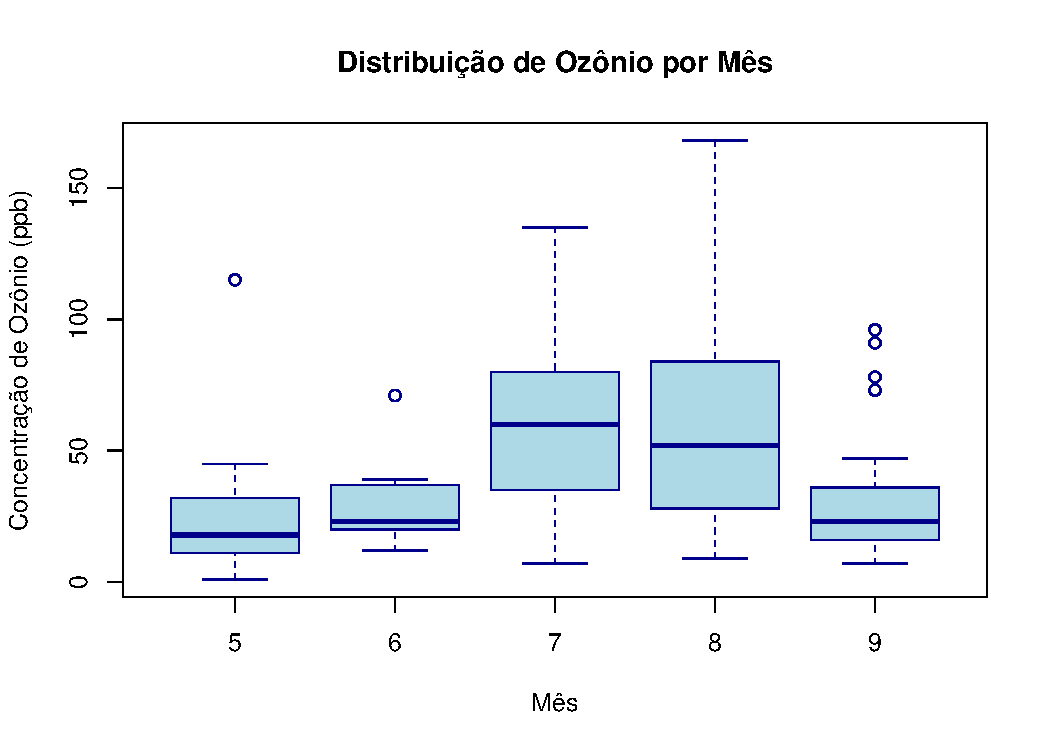
\includegraphics[width=0.75\textwidth]{figura.pdf}
  \caption{Distribuição dos níveis de ozônio entre os meses 5 e 9.}
  \label{fig:distribuicao}
\end{figure}

\section*{Declaração de uso de IA}

Utilizou-se o assistente Gemini para apoio na verificação das rotinas em terminal Unix. Verifcação dos cálculos e  dados numéricos, conferência e alguma correções dos códigos gerados.

\bibliographystyle{plainnat}
\bibliography{referencias}

\end{document}
